% =====================================================================
% ejercicio10.tex
% Responsabilidad única: registrar los candidatos congelados, evaluarlos una única vez en prueba
% y redactar la recomendación final.
% Las cifras provienen de generado/resultados.tex y generado/tabla_*.tex.
% =====================================================================
\subsection{Ejercicio 10: Evaluación final y recomendación sustentada}

Antes de abrir la prueba dejamos registrados los candidatos finales
(Tabla~\ref{tab:ex10-candidatos}), ambos con todos los predictores de su
caso, y conservamos los modelos tal como quedaron ajustados con
entrenamiento.

\begin{table}[H]
\centering
\resizebox{\textwidth}{!}{% Archivo generado automáticamente por el notebook (no editar a mano).
\begin{tabular}{lllll}
\toprule
Caso & Candidato final & Hiperparámetros & Umbral & Criterio de validación \\
\midrule
A (regresión) & Regresión múltiple (10 predictores) & StandardScaler + LinearRegression & — & RMSE = 51.1937 \\
B (clasificación) & Regresión logística (C = 1) & StandardScaler + LogisticRegression(C=1, lbfgs, L2) & 0.7 & L = 5 \\
\bottomrule
\end{tabular}
}
\caption{Candidatos finales congelados, decididos con validación.}
\label{tab:ex10-candidatos}
\end{table}

\begin{enumerate}

\item \textbf{Regresión en prueba.}

\begin{table}[H]
\centering
\resizebox{\textwidth}{!}{% Archivo generado automáticamente por el notebook (no editar a mano).
\begin{tabular}{lrrrrl}
\toprule
Modelo & MAE & RMSE & $R^2$ & RMSE val. & Elegido \\
\midrule
Constante (media) & 63.5314 & 72.9002 & $-$0.0031 & 75.6392 &  \\
Regresión simple (bmi) & 51.9829 & 63.8336 & 0.2309 & 58.5671 &  \\
Regresión múltiple (10 predictores) & 42.9245 & 54.1564 & 0.4464 & 51.1937 & $\checkmark$ \\
Árbol (max\_depth=4, min\_samples\_leaf=30) & 44.8448 & 58.2134 & 0.3604 & 56.7789 &  \\
\bottomrule
\end{tabular}
}
\caption{Modelos de regresión en prueba, con el RMSE de validación como referencia.}
\label{tab:ex10-reg}
\end{table}

La regresión múltiple siguió siendo la mejor en prueba (RMSE de
$\TestMultiRMSE$ y $R^2$ de $\TestMultiRdos$), seguida del árbol
($\TestArbolRegRMSE$), el modelo simple ($\TestSimpleRMSE$) y la constante
($\TestDummyRMSE$), el mismo orden que en validación
(Tabla~\ref{tab:ex10-reg}). El candidato elegido pasó de un RMSE de
validación de $\CandidatoRegRMSEVal$ a uno de prueba de
$\CandidatoRegRMSETest$, y su $R^2$ de $\RegMultiRdosVal$ a
$\TestMultiRdos$. Esa caída no nos tomó por sorpresa, porque desde el
Ejercicio~6 habíamos notado que la validación resultó una partición algo más
favorable para todos los modelos, y en cualquier caso no cambiamos de
candidato a la luz de estos resultados.

\item \textbf{Clasificación en prueba.}

\begin{table}[H]
\centering
\small
% Archivo generado automáticamente por el notebook (no editar a mano).
\begin{tabular}{llrrrr}
\toprule
Modelo & Umbral & Precisión & Recall & F1 & ROC-AUC \\
\midrule
Referencia (prior) & 0.5 & 0.0000 & 0.0000 & 0.0000 & 0.5000 \\
Regresión logística (C = 1) & 0.7 & 1.0000 & 0.9286 & 0.9630 & 0.9954 \\
Árbol (max\_depth=3, min\_samples\_leaf=15) & 0.2 & 0.8542 & 0.9762 & 0.9111 & 0.9730 \\
\bottomrule
\end{tabular}

\caption{Clasificación en prueba con los umbrales congelados: métricas.}
\label{tab:ex10-clf-met}
\end{table}

\begin{table}[H]
\centering
\small
% Archivo generado automáticamente por el notebook (no editar a mano).
\begin{tabular}{llrrrrr}
\toprule
Modelo & Umbral & TN & FP & FN & TP & Costo L \\
\midrule
Referencia (prior) & 0.5 & 72 & 0 & 42 & 0 & 210 \\
Regresión logística (C = 1) & 0.7 & 72 & 0 & 3 & 39 & 15 \\
Árbol (max\_depth=3, min\_samples\_leaf=15) & 0.2 & 65 & 7 & 1 & 41 & 12 \\
\bottomrule
\end{tabular}

\caption{Clasificación en prueba con los umbrales congelados: errores y costo $L=FP+5FN$.}
\label{tab:ex10-clf-cost}
\end{table}

La regresión logística con $t=\LogitT$ obtuvo en prueba precisión
$\TestLogitPrec$, recall $\TestLogitRecall$, F1 $\TestLogitFUno$ y ROC-AUC
$\TestLogitAUC$, con $FP=\TestLogitFP$ y $FN=\TestLogitFN$
($L=\TestLogitCosto$), mientras que el árbol con $t=\ArbolT$ obtuvo
precisión $\TestArbolClfPrec$, recall $\TestArbolClfRecall$, F1
$\TestArbolClfFUno$ y ROC-AUC $\TestArbolClfAUC$, con $FP=\TestArbolClfFP$ y
$FN=\TestArbolClfFN$ ($L=\TestArbolClfCosto$); la referencia predice todo
benigno y acumuló $L=\TestDummyCosto$. Aquí vino la parte incómoda: en
prueba el árbol tuvo un costo algo menor que el candidato elegido. La
diferencia se explica por los falsos negativos adicionales de la logística,
compensados solo en parte por sus menos falsos positivos, y coincide con la
advertencia que dejamos en el Ejercicio~8c sobre un umbral alto elegido con
pocos malignos de validación. Lo discutimos y decidimos mantener el
candidato, pues la decisión la tomamos con validación y cambiarla ahora
sería usar la prueba para seleccionar; además, con $\NClfTest$ muestras una
diferencia de pocas unidades de costo es compatible con la variabilidad
muestral, y la logística conserva un ROC-AUC claramente superior.

\paragraph{Incertidumbre de la evaluación final.}
No quisimos quedarnos solo con afirmar esa variabilidad, así que la
cuantificamos: remuestreamos con reemplazo cada conjunto de prueba
($B=\BootB$ réplicas, semilla $\Semilla$) recalculando las métricas con las
\emph{mismas predicciones congeladas}, sin reajustar nada, y comparamos los
modelos mediante diferencias \emph{pareadas} (ambos evaluados sobre la misma
réplica), que descuentan la variabilidad común (Tabla~\ref{tab:ex10-boot} y
Figura~\ref{fig:ex10-boot}).

\begin{table}[H]
\centering
\small
% Archivo generado automáticamente por el notebook (no editar a mano).
\begin{tabular}{lrrr}
\toprule
Cantidad & Puntual & IC 95 \% inf. & IC 95 \% sup. \\
\midrule
RMSE regresión múltiple & 54.1564 & 46.4859 & 61.7067 \\
RMSE árbol de regresión & 58.2134 & 49.0516 & 66.7298 \\
RMSE regresión simple & 63.8336 & 55.0919 & 72.5263 \\
$\Delta$ RMSE múltiple $-$ árbol & $-$4.0570 & $-$12.2259 & 3.5369 \\
$\Delta$ RMSE múltiple $-$ simple & $-$9.6771 & $-$17.5818 & $-$2.0302 \\
ROC-AUC logística & 0.9954 & 0.9839 & 1.0000 \\
ROC-AUC árbol & 0.9730 & 0.9410 & 0.9960 \\
Costo L logística & 15 & 0 & 35 \\
Costo L árbol & 12 & 3 & 24 \\
$\Delta$ L logística $-$ árbol & 3 & $-$16 & 27 \\
\bottomrule
\end{tabular}

\caption{Intervalos bootstrap percentiles al 95\,\% en prueba
($B=\BootB$, predicciones congeladas).}
\label{tab:ex10-boot}
\end{table}

\begin{figure}[H]
    \centering
    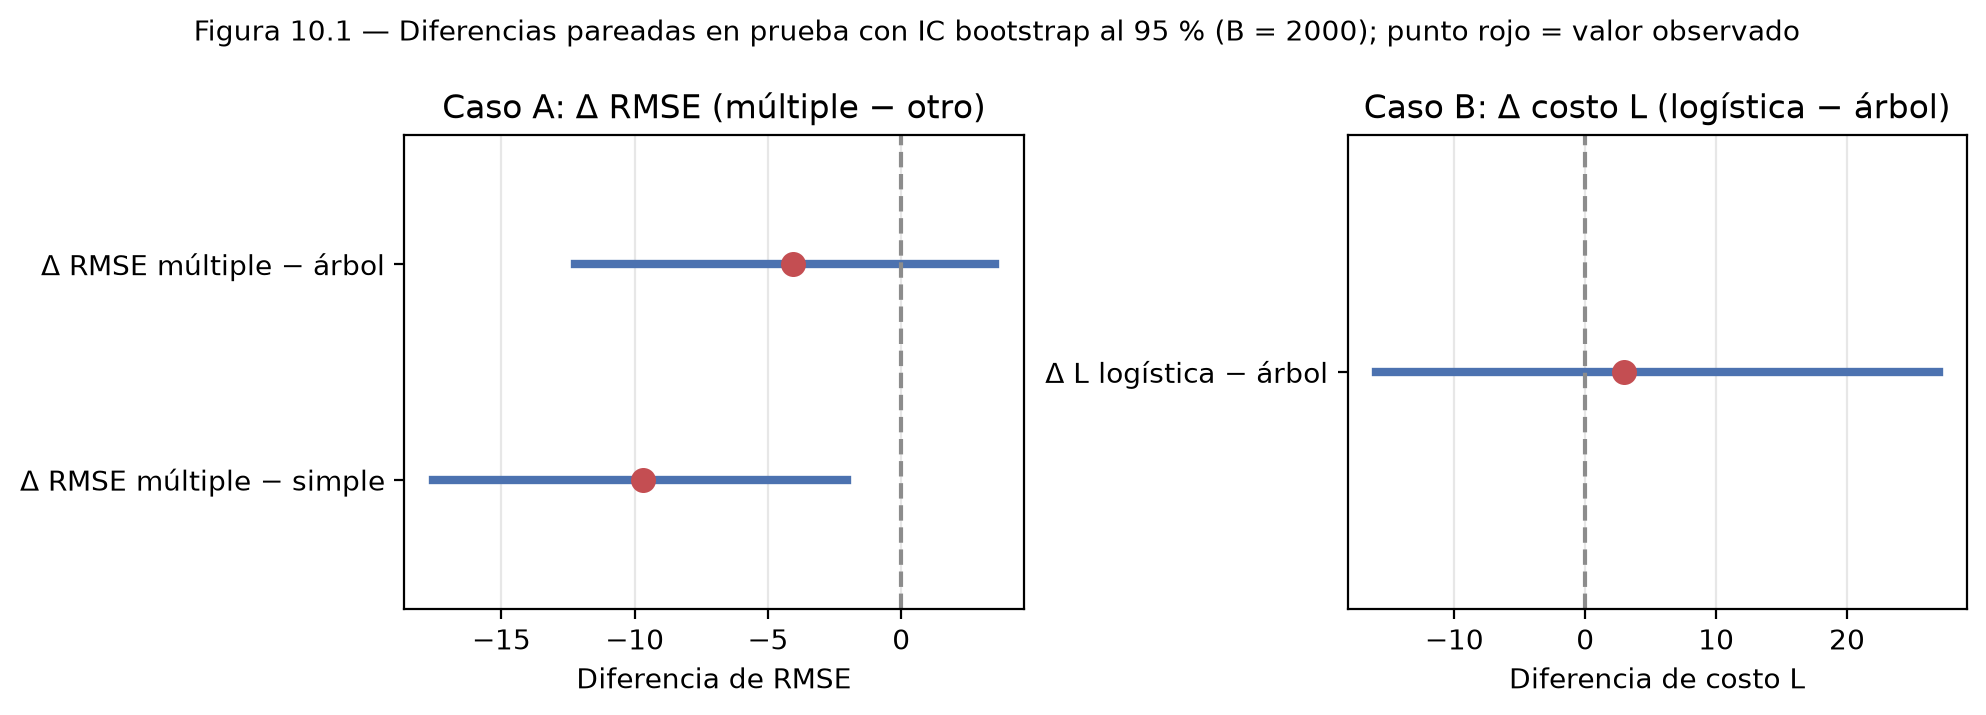
\includegraphics[width=\textwidth]{figuras/ex10_bootstrap.png}
    \caption{Diferencias pareadas en prueba con su intervalo bootstrap al
    95\,\%; si el intervalo cruza la línea punteada (cero), la prueba no
    permite distinguir a los dos modelos.}
    \label{fig:ex10-boot}
\end{figure}

En el caso A la regresión múltiple superó a la simple con un intervalo para
la diferencia de RMSE de $[\BootDifRMSEMultiSimpleInf,\ \BootDifRMSEMultiSimpleSup]$,
que excluye el cero, de forma que esa mejora es robusta, mientras que frente
al árbol el intervalo $[\BootDifRMSEMultiArbolInf,\ \BootDifRMSEMultiArbolSup]$
sí incluye el cero, por lo cual la prueba por sí sola no nos permite afirmar
que la múltiple sea mejor que el árbol (la elección se sostiene en la
validación y en su menor complejidad). En el caso B la diferencia pareada de
costo (logística menos árbol) fue de $\BootDifLLogitArbolInf$ a
$\BootDifLLogitArbolSup$, con la logística más costosa en una fracción
$\BootPropLogitPeor$ de las réplicas, es decir, la ventaja del árbol en
prueba es compatible con el azar del muestreo, mientras que la superioridad
de la logística en ordenamiento es más clara (ROC-AUC con intervalo
$[\BootAUCLogitInf,\ \BootAUCLogitSup]$ frente a
$[\BootAUCArbolInf,\ \BootAUCArbolSup]$ del árbol). Los intervalos de $L$
salieron tan anchos porque $L$ depende de unos pocos falsos negativos que
valen 5 cada uno.

\item \textbf{Matrices de confusión y costo.}

\begin{figure}[H]
    \centering
    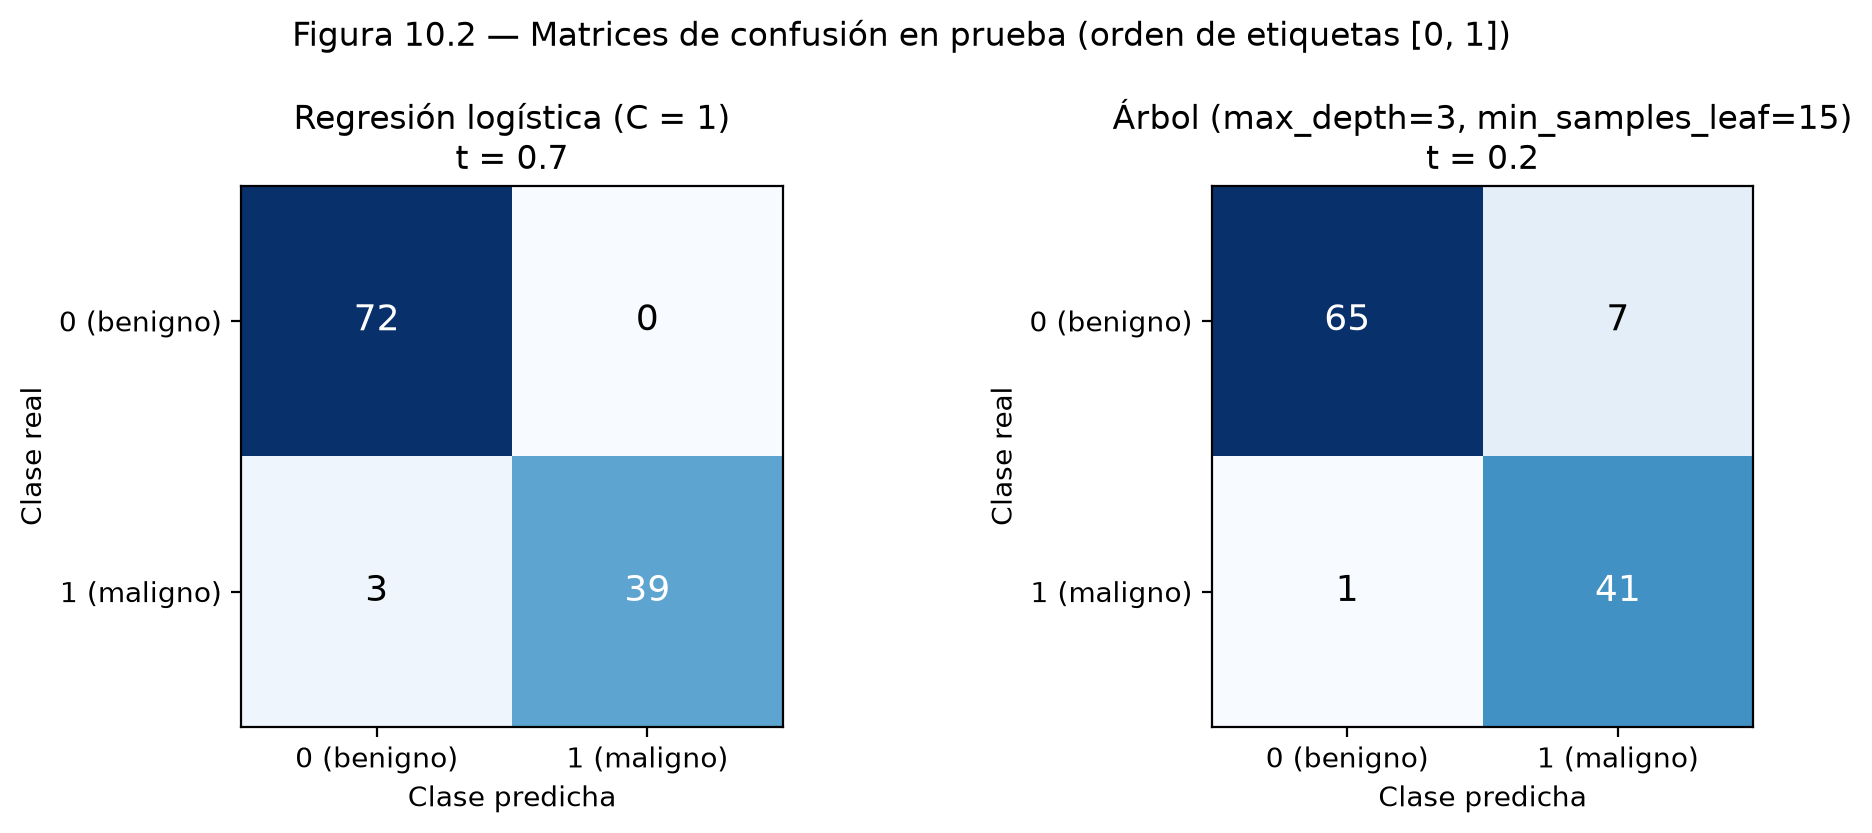
\includegraphics[width=\textwidth]{figuras/ex10_matrices_confusion.png}
    \caption{Matrices de confusión en prueba, filas reales y columnas predichas en orden $[0,1]$.}
    \label{fig:ex10-cm}
\end{figure}

En este conjunto, un \textbf{falso positivo} es una muestra de tejido
benigno clasificada como maligna, lo que en un uso hipotético implicaría
exámenes adicionales innecesarios y angustia para la paciente, mientras que
un \textbf{falso negativo} es una muestra maligna clasificada como benigna,
lo que retrasaría un diagnóstico y un tratamiento, consecuencia mucho más
grave y razón por la cual el costo didáctico la pondera cinco veces. Para el
candidato elegido, la matriz de la Figura~\ref{fig:ex10-cm} quedó con
$TN=\TestLogitTN$, $FP=\TestLogitFP$, $FN=\TestLogitFN$ y $TP=\TestLogitTP$,
de modo que
\[
    L = FP + 5\,FN = \TestLogitFP + 5\cdot\TestLogitFN = \TestLogitCosto,
\]
valor que coincide con la Tabla~\ref{tab:ex10-clf-cost}.

\item \textbf{Recomendación.}
% Versión en primera persona del texto de la celda 10d del notebook (allí
% se verifica el rango exigido de 250 a 350 palabras).
Para el caso A (progresión de la diabetes) recomendamos la regresión lineal
múltiple con los diez predictores estandarizados, pues fue el candidato con
menor RMSE de validación ($\CandidatoRegRMSEVal$) y conservó el primer lugar
en prueba (RMSE de $\TestMultiRMSE$ y $R^2$ de $\TestMultiRdos$), por delante
del árbol y de la regresión simple con \texttt{bmi}. Además es interpretable,
ya que cada coeficiente se lee como el cambio esperado ante una desviación
estándar del predictor, con el detalle de que la fuerte correlación entre
\texttt{s1} y \texttt{s2} impide leer esos coeficientes como importancias
independientes o como efectos causales, y un $R^2$ cercano a
$\TestMultiRdos$ indica que más de la mitad de la variabilidad queda sin
explicar.

Para el caso B (clasificación de tejido) recomendamos la regresión logística
con $C=\LogitC$ y umbral $\LogitT$, que elegimos por menor costo en
validación ($L=\LogitCostoSel$) y que en prueba obtuvo ROC-AUC de
$\TestLogitAUC$, precisión de $\TestLogitPrec$ y recall de
$\TestLogitRecall$, aunque con $L=\TestLogitCosto$ frente a
$L=\TestArbolClfCosto$ del árbol, diferencia que con $\NClfTest$ muestras de
prueba no justifica cambiar de candidato después de ver los resultados. El
árbol, más simple de explicar con dos o tres reglas, sacrifica capacidad de
ordenamiento y depende de pocas variables.

Si un candidato rinde peor en prueba que en validación, como nos pasó en
ambos casos, lo reportamos tal cual como estimación honesta y, en lugar de
reajustar con prueba, revisamos el análisis sobre el conjunto de desarrollo
y, de ser necesario, reservamos un nuevo conjunto de prueba.

Nos quedan dos limitaciones. Primero, los tamaños son pequeños ($\NRegVal$ y
$\NClfVal$ observaciones de validación), por lo que umbrales y empates
dependen de unos pocos casos. Segundo, los datos son observacionales y de
una sola fuente, sin evaluación externa ni costos clínicos reales detrás de
$L=FP+5FN$. Como mejora futura proponemos elegir hiperparámetros y umbral con
validación cruzada estratificada dentro del conjunto de desarrollo, menos
sensible a una sola partición, y luego evaluar en una cohorte externa.

\end{enumerate}
